% !TEX encoding = UTF-8 Unicode
%!TEX root = thesis.tex
% !TEX spellcheck = en-US
%%=========================================
\chapter{Method}
\label{chap:chapter3}

To fulfill the goal of this thesis, an experiment to compare the energy use of different JavaScript engines was developed:
Measuring the current drawn while executing benchmark programs in different JavaScript engines on various hardware platforms
These measurements can be used to find the power used by a single expression.
By running the programs a large number of times, an average power consumption of the expressions can be obtained.
All of the programs are trivial operations in a loop, and by calculating the average consumption the energy cost of a single expression in the JavaScript engine can be found.

The experiment will look at three different software solutions to execute JavaScript code, each with its own implementation tactic, namely Tessel, Espruino and io.js.
They are used on two different hardware platforms, the Tessel and the Raspberry Pi 1 Model B.

The goal of the experiment is to look at differences in the energy use of the different JavaScript implementations.
This means that it is not the exact numbers that are of interest, but rather the trends.

\section{Benchmarks}
Four programs were used as benchmarks on each tested platform, all following a similar pattern: In a loop repeated 1,000,000 times, an expression is evaluated.
The programs are named after the expression used in it, testing various JavaScript features; namely Addition, Multiplication, Closure, and Left shift.
The addition program can be seen in \cref{lst:add}, and the multiplication program in \cref{lst:multi}.
The expression evaluated in these two are basic instructions, which virtually every language contains.

\begin{figure}[h!]
\begin{minipage}{0.45\textwidth}
\begin{minted}{js}
for(var i = 0; i < 1000000; i++) {
    var a = 1;
    var b = 2;
    var c = a + b;
}
\end{minted}
\captionof{listing}{The Addition program}
\label{lst:add}
\end{minipage}\hfill
\begin{minipage}{0.45\textwidth}
\begin{minted}{js}
for(var i = 0; i < 1000000; i++) {
    var a = 1;
    var b = 2;
    var c = a * b;
}
\end{minted}
\captionof{listing}{The Multiplication program}
\label{lst:multi}
\end{minipage}
\end{figure}

\begin{figure}[h!]
\begin{minipage}{0.45\textwidth}
\begin{minted}{js}
for(var i = 0; i < 1000000; i++) {
    var a = 1;
    var b = 2;
    var c = a << b;
}
\end{minted}
\captionof{listing}{The Left shift program}
\label{lst:shift}
\end{minipage}\hfill
\begin{minipage}{0.45\textwidth}
\begin{minted}{js}
for(var i = 0; i < 1000000; i++) {
    var a = 1;
    var c = (function () {return a})();
}
\end{minted}
\captionof{listing}{The Closure program}
\label{lst:closure}
\end{minipage}
\end{figure}

In \cref{lst:shift}, the Left shift program is shown.
Like the addition and multiplication program, it consists of a single expression, a left shift.
To left shift \emph{a} by \emph{b} is to add b zeros to the end of a's binary representation.
For example:
\[1_{10} << 2_{10} = 1_{2} << 10_{2} = 100_{2} = 4_{10}\]

The Closure program, seen in \cref{lst:closure}, evaluates a \emph{closure}, which accesses a global variable.
A closure is a concept often used in JavaScript programs, where an unnamed local function is evaluated where it is defined.
In this example it may seem trivial, but as JavaScript only has a scope per function, closures are an important tool to not clutter the global scope.
And with the single threaded nature of the language, as well as its higher order, closures are an important flow control concept in applications.




\section{Hardware Platforms}

\begin{figure}[h!]
\centering
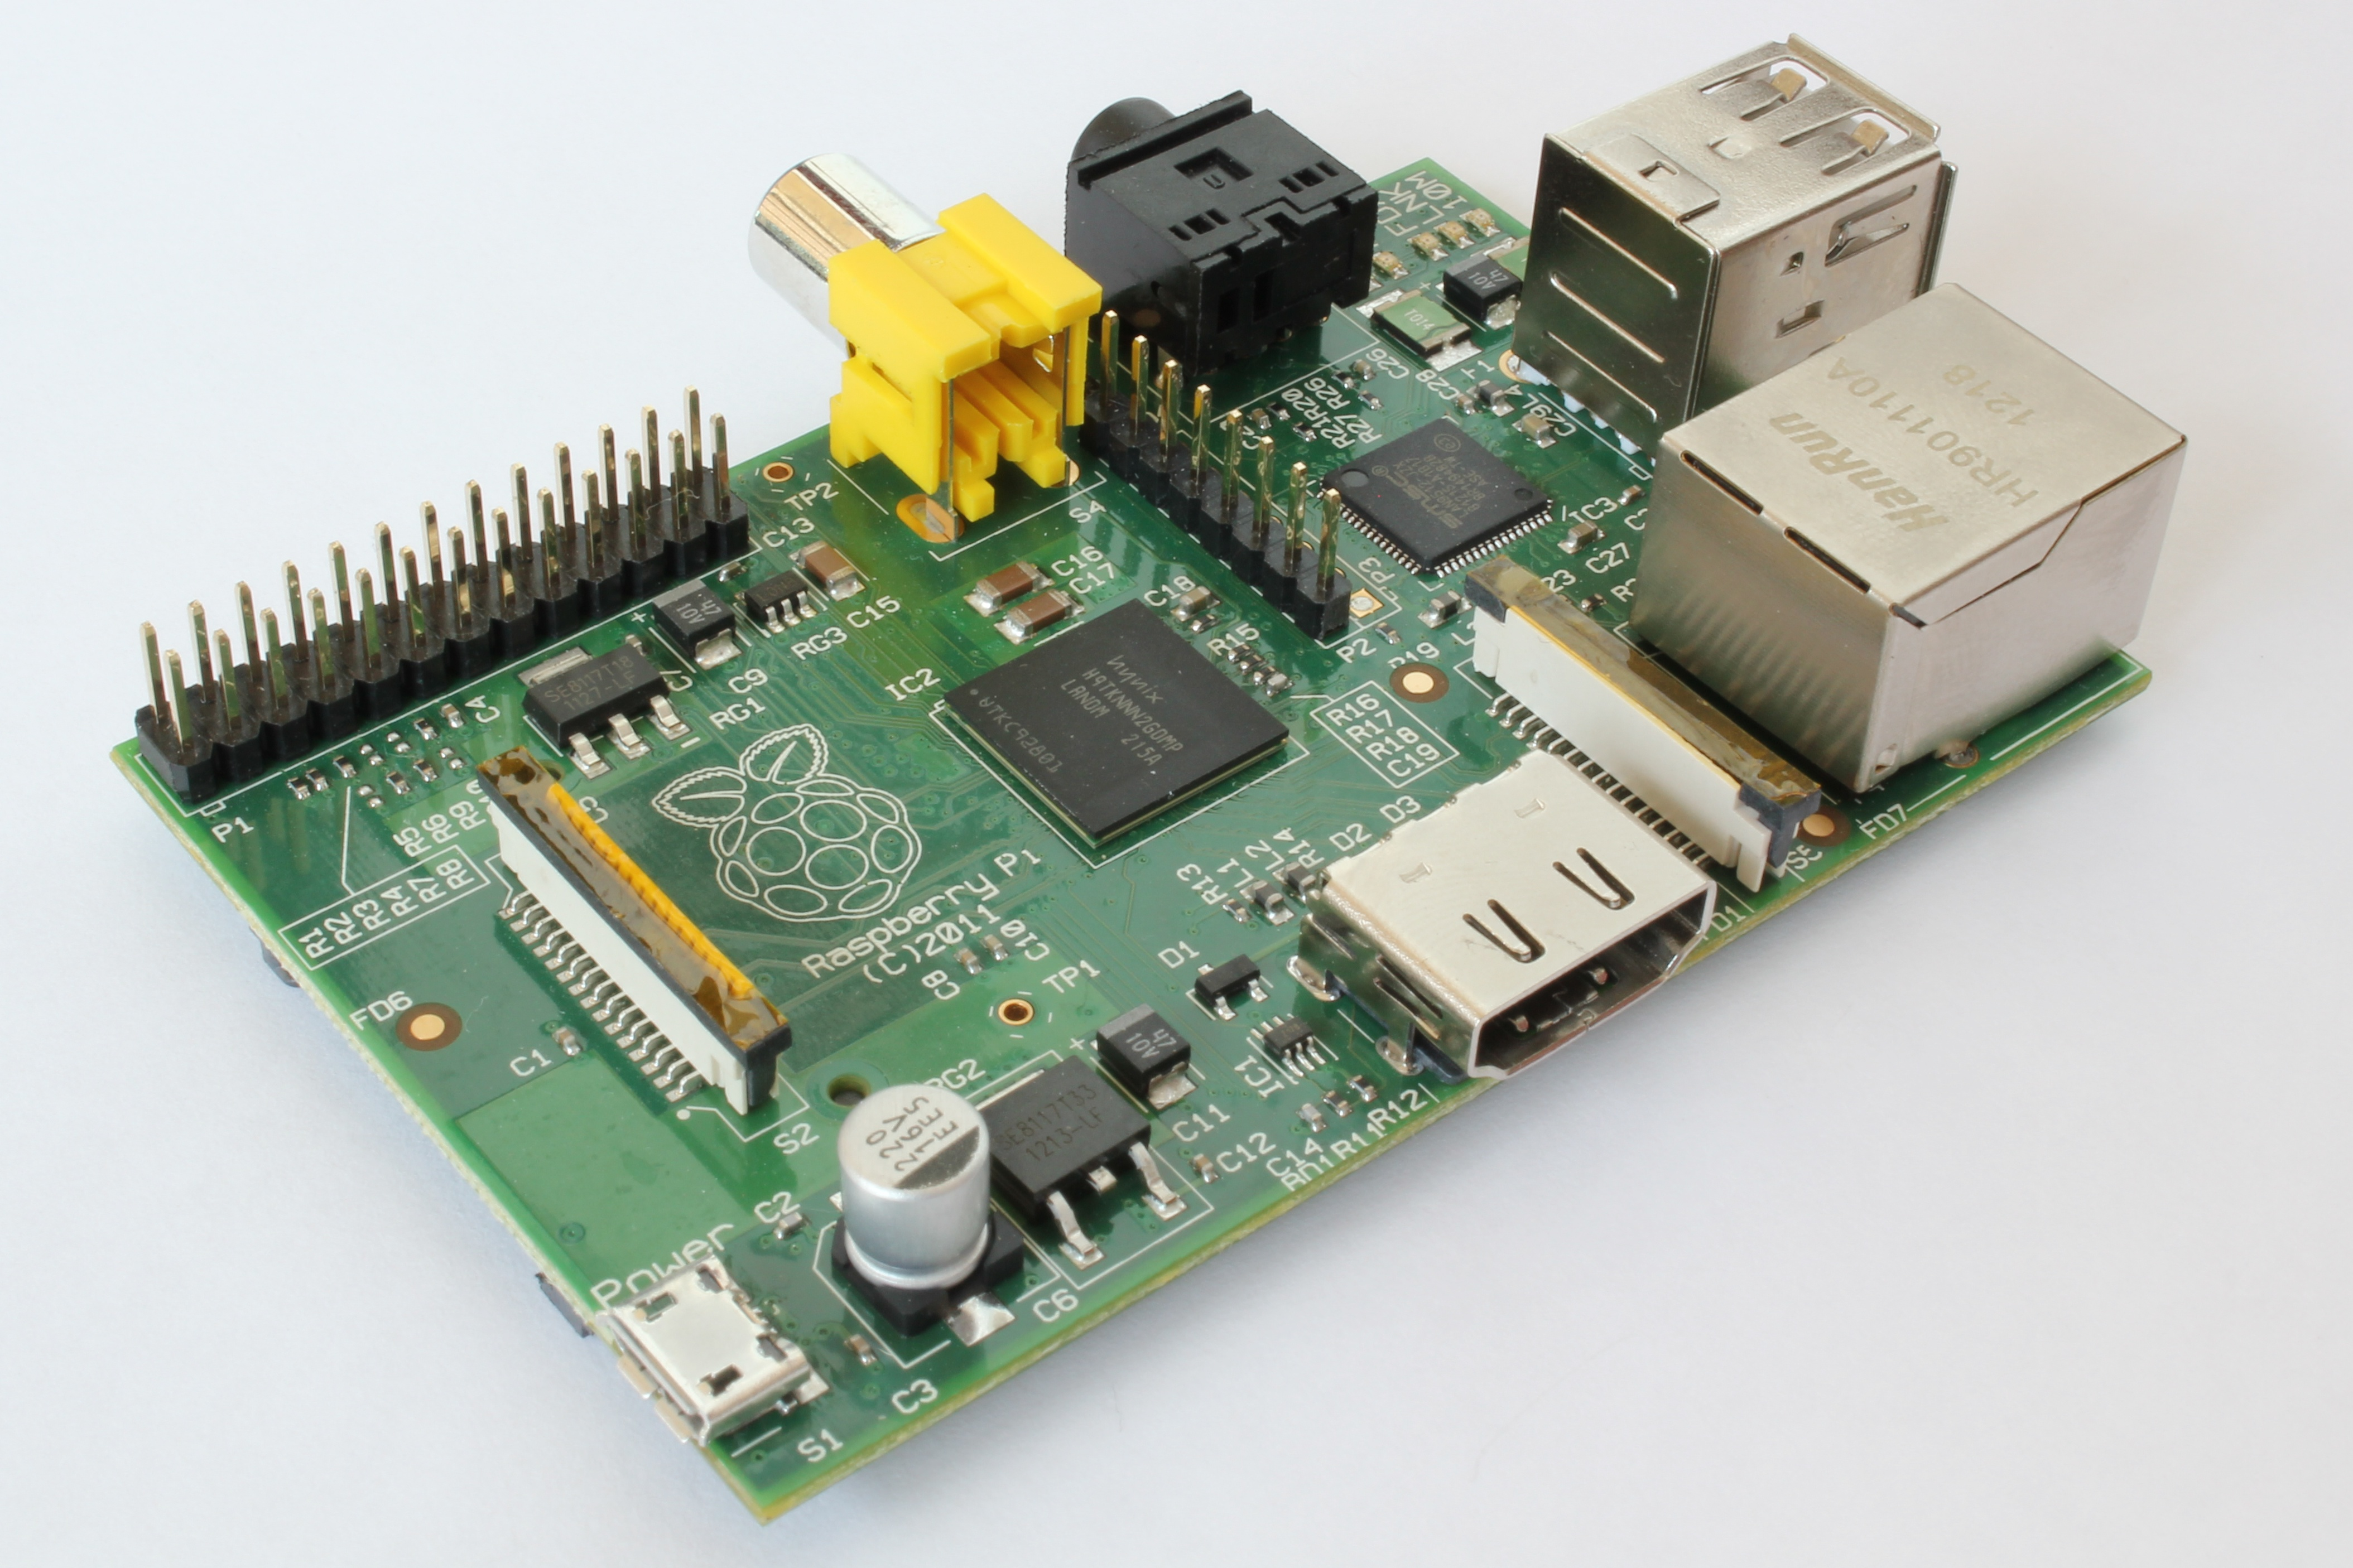
\includegraphics[scale=0.08]{fig/pics/RaspberryPi.jpg}
\caption{Raspberry Pi Model B, {\tiny source: \url{https://commons.wikimedia.org/wiki/File:RaspberryPi.jpg}}}
\label{fig:raspberrypi}
\end{figure}

\begin{figure}[h!]
\centering
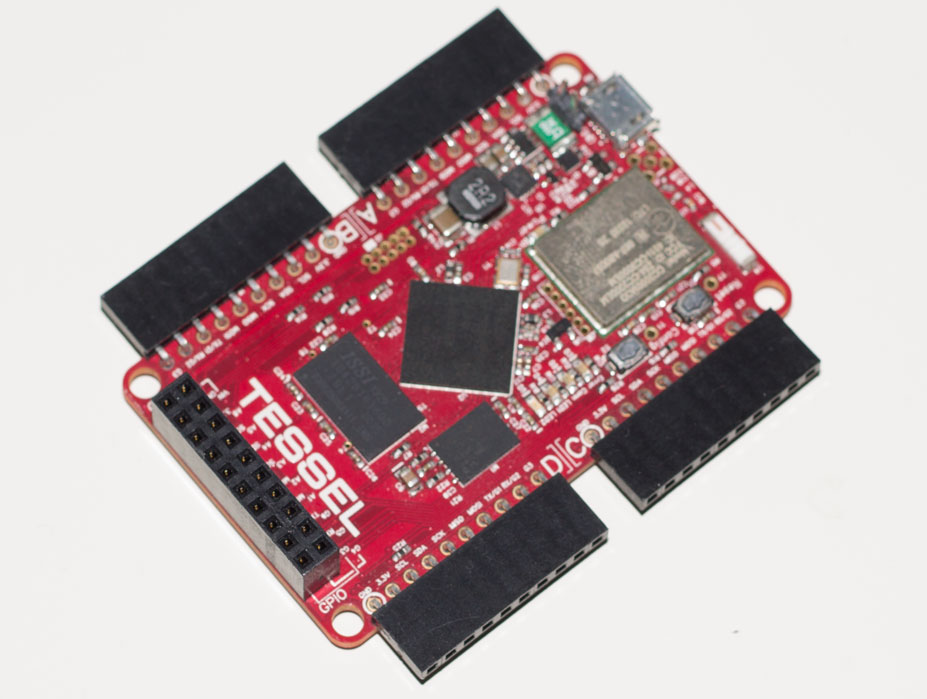
\includegraphics[scale=0.4]{fig/pics/tessel.jpg}
\caption{The Tessel 1}
\label{fig:tessel}
\end{figure}
\defcitealias{tesselhardware}{Tessel Harwdare Documentation}
\newcolumntype{A}{>{\columncolor[gray]{.9}}c}
\newcolumntype{B}{>{\columncolor[gray]{.8}}c}
\begin{table}[h]
\centering
\begin{tabular}{ c B  A }
            & Raspberry Pi  & Tessel        \\ 
CPU         & BCM2835       & LPC1830       \\ 
Core        & ARM1173       & ARM Cortex M3 \\ 
Architecture& ARMv6         & ARMv7         \\ 
Clock Speed & 700 \si{\mega\hertz}& 180 \si{\mega\hertz}\\ 
RAM         & 512 MB & 32 MB\\ 
Flash       & SD-card       & 32 MB\\
\end{tabular}
\caption{Comparing a Tessel 1 with a Raspberry Pi 1 Model B \citepalias{tesselhardware}}
\label{tab:specs}
\end{table}
\todo{sources on specs of Raspberry Pi}


As can be gathered from \cref{tab:specs}, the Raspberry Pi is a much faster machine than the Tessel, clocked at almost 4 times higher, and with 16 times the amount of RAM.
This means that the Raspberry Pi is able to run much larger software and do it faster, but also that it will use more power.

\subsection{Silicon Labs EFM32 Giant Gecko}

\begin{table}[h!]
\centering
\begin{tabular}{c A}
CPU & GG990 \\
Core & ARM Cortex M3\\
Architecture & ARMv7 \\
Clock speed & 48\si{\mega\hertz} \\
RAM & 128KB KB \\
Flash & 1024 KB
\end{tabular}
\caption{Key data of the Giant Gecko 990 \citepalias{efm32gg990ds}}
\label{tab:ggkeydata}
\end{table}

When developing the experiment, another hardware platform was intended to be tested.
The Giant Gecko from Silicon Labs is a microcontroller created for low energy use cases, which is described in \cref{sec:hwenergy}.
\todo{better}To develop on the platform, the development board EFM32GG-DK3750 was used.
It uses the CPU which is described in \cref{tab:ggkeydata}.
It is a much less powerful device than both the Tessel and the Raspberry Pi, clocked at a third of the Tessel, and containing a small fraction of the memory available on the other platforms.

\section{Software Platforms}
\subsection{Tessel}
\defcitealias{newengine}{A New Engine For Your Tessel, 2014}
\defcitealias{movingfaster}{Moving Faster With io.js, 2015}
\defcitealias{aboutlua}{About Lua}

Tessel\footnote{https://tessel.io}, developed by Technical Machine, is a project created for offering software developers a platform for developing hardware for the first time.
It consists of both a hardware platform, described above, and a software platform.
This software platform includes a runtime for the hardware, interpreting the code, a command line interface to easily run programs, and a compiler.
Instead of interpreting JavaScript, Tessel compiles it to Lua, and interprets the Lua code on the device.

\emph{Lua} is another programming language, designed to be fast and lightweight, and is easily embeddable. In many ways, it is similar to JavaScript, so a translation from JavaScript to Lua is not very difficult. There exists two main implementations of Lua, the official interpreter, and LuaJIT, a highly optimized just-in-time compilator and virtual machine.\citepalias{aboutlua}

One of the rationales behind choosing Lua as the intermediate language was that Lua has a low memory profile and is easy to embed.
The alternative when Tessel was first envisioned, was using the V8 engine, in the same way io.js do.
But at the time, Technical Machine did not think V8 could be reconciled with the low power goals they had for the Tessel.
To further drive down energy use, the LuaJIT compiler was introduced, first only the virtual machine, but with the goal of enabling just-in-time compilation in the future. \citepalias{newengine}

The compiler of the Tessel, the Colony Compiler\footnote{https://github.com/tessel/colony-compiler}, is a simple lexical parser, that translates the JavaScript expressions into the Lua equivalents.
This means that while a complete compilation of the source code is done, it does not do any optimizations to the output.

In newer developments, the developers of Tessel have found out that some of the goals of the Tessel project can’t be reconciled with a real low power usage, therefore the next version of Tessel will run io.js, using a Linux based operating system.\citepalias{movingfaster}

\subsection{Espruino}
\defcitealias{espruinoperf}{Espruino Performance Notes}
\defcitealias{epsruinointern}{Espruino Interpreter Internals}
Espruino\footnote{http://www.espruino.com/} is another project that aims to bring hardware to software developers, also through JavaScript.
But unlike Tessel, the goal is to target devices with memory as small as 128kB Flash and 8kB RAM.
The Espruino project consists of both a software and a hardware platform, but to achieve the low memory goal, the software implementation includes a lot of trade-offs.

The Espruino virtual machine (VM) is an almost complete JavaScript implementation, where the difference between this and other JavaScript implementations being that Espruino does not translate the source code to byte code, but executes the source directly, one expression at a time.
This is again due to memory concerns, as the developers want the source code to be on the device when executing, to be able to edit the source code on the device. 
If the VM translated to intermediate byte code, it would need twice the amount of storage for the same program to keep it all on the device.\citepalias{epsruinointern}

Other optimizations done for memory minimization include using a linked list for storage of arrays and objects (allowing for constant time insertion and deletion) and including typed arrays, which is a direct mapping of memory to the data structure.\citepalias{espruinoperf}

While the platform itself is designed to be power efficient, it does not optimize the code before running it, requiring the programmer to write efficient code.

\subsection{io.js}
\defcitealias{aboutnodejs}{About Node.js}
io.js\footnote{https://iojs.org} is a framework created with the goal of using the V8 JavaScript engine without a browser, and with a rich input and output(I/O) API.
The framework is asynchronous and event driven, designed for creating scalable network applications.
The io.js framework uses an event loop that runs callbacks, functions that are registered to be run when an arbitrary event happens.
This makes io.js different from traditional thread based programming platforms, where I/O blocks further execution of the code.\citepalias{aboutnodejs}

But as a wrapper around V8, io.js also functions as an easy way of installing a JavaScript runtime on computers, allowing JavaScript to be used as an alternative to other programming languages.

io.js is a fork of Node.js, with a different development schedule and philosophy.
Currently, io.js uses a newer version of the V8 engine than Node.js.
But the io.js team has recently announced that they will be joining the new Node Foundation, and the project that is currently io.js, will be renamed Node. in the near future.\footnote{https://medium.com/node-js-javascript/io-js-week-of-may-15th-9ada45bd8a28}
This makes the terminology in this thesis a bit hard, as the project may suddenly have changed name.
But as the future Node.js will be more or less based upon the as of writing io.js project, the least confusing wording is to use io.js consistently.

\subsubsection{V8}
\defcitealias{v8designelements}{V8 Design Elements}
Used in io.js, is the V8 JavaScript engine built by Google, and used in the Google Chrome Web Browser.
The development is done with a focus on creating the fastest JavaScript engine possible.
It outperforms all other major JavaScript engines available today.
To be this fast, there are three major design areas \citepalias{v8designelements}:

\emph{Fast property access}, as JavaScript is a dynamic language, property access usually is slow, due to it requiring a dictionary lookup.
V8 uses dynamically created hidden classes to be able to access properties from offsets, requiring a single load instruction.
It only requires these classes to be created once for each object, which leads to faster creation of any other objects of the same class.

\emph{Dynamic machine code generation}, the engine uses just-in-time compilation, directly to byte code.
Because of the hidden classes created for the fast property access, the compiler can guess that after property access, the current class will be used for all future accesses in the same section of code.

\emph{Efficient garbage collection}, V8 uses a strategy for memory reclaiming that is aimed at running for as short time as possible. To do this, it stops program execution when performing garbage collection and does not process the whole heap in most collection cycles.


\subsection{Operating system}
To run programs on a computer, some sort of operating system is needed to control the input and output mechanisms, and schedule which program is to run.
The Tessel 1 firmware includes a basic OS, so the developer does not need to do anything special.

On the Raspbery Pi, an operating system needs to be installed.
Provided from the website is the Raspbian Linux distribution, based on Debian 7.
Since the Raspberry Pi has an ARMv6 processor, but Debian only supports ARMv7 natively, this distribution was created separately.
But Raspbian is not actively maintained, and has become quite outdated.
Debian is currently in version 8.
% http://sjoerd.luon.net/posts/2015/02/debian-jessie-on-rpi2/

To get an operating system on the Giant Gecko, uClinux through the PTXdist build system.
It consists of a complete toolchain for building Linux, and a lot of rules to build packages for various systems, among them the Giant Gecko DK3750.\footnote{http://git-public.pengutronix.de/?p=OSELAS.BSP-EnergyMicro-Gecko.git}
It is not a distribution, but an ``executable documentation'', in that it contains the steps necessary to build the target system in scripts that can be read or executed.\citep{ptxdistguru}

\section{Experimental setup}
\missingfigure{schematic of experiment}
\label{sec:expsetup}
\begin{figure}[h!]
\centering
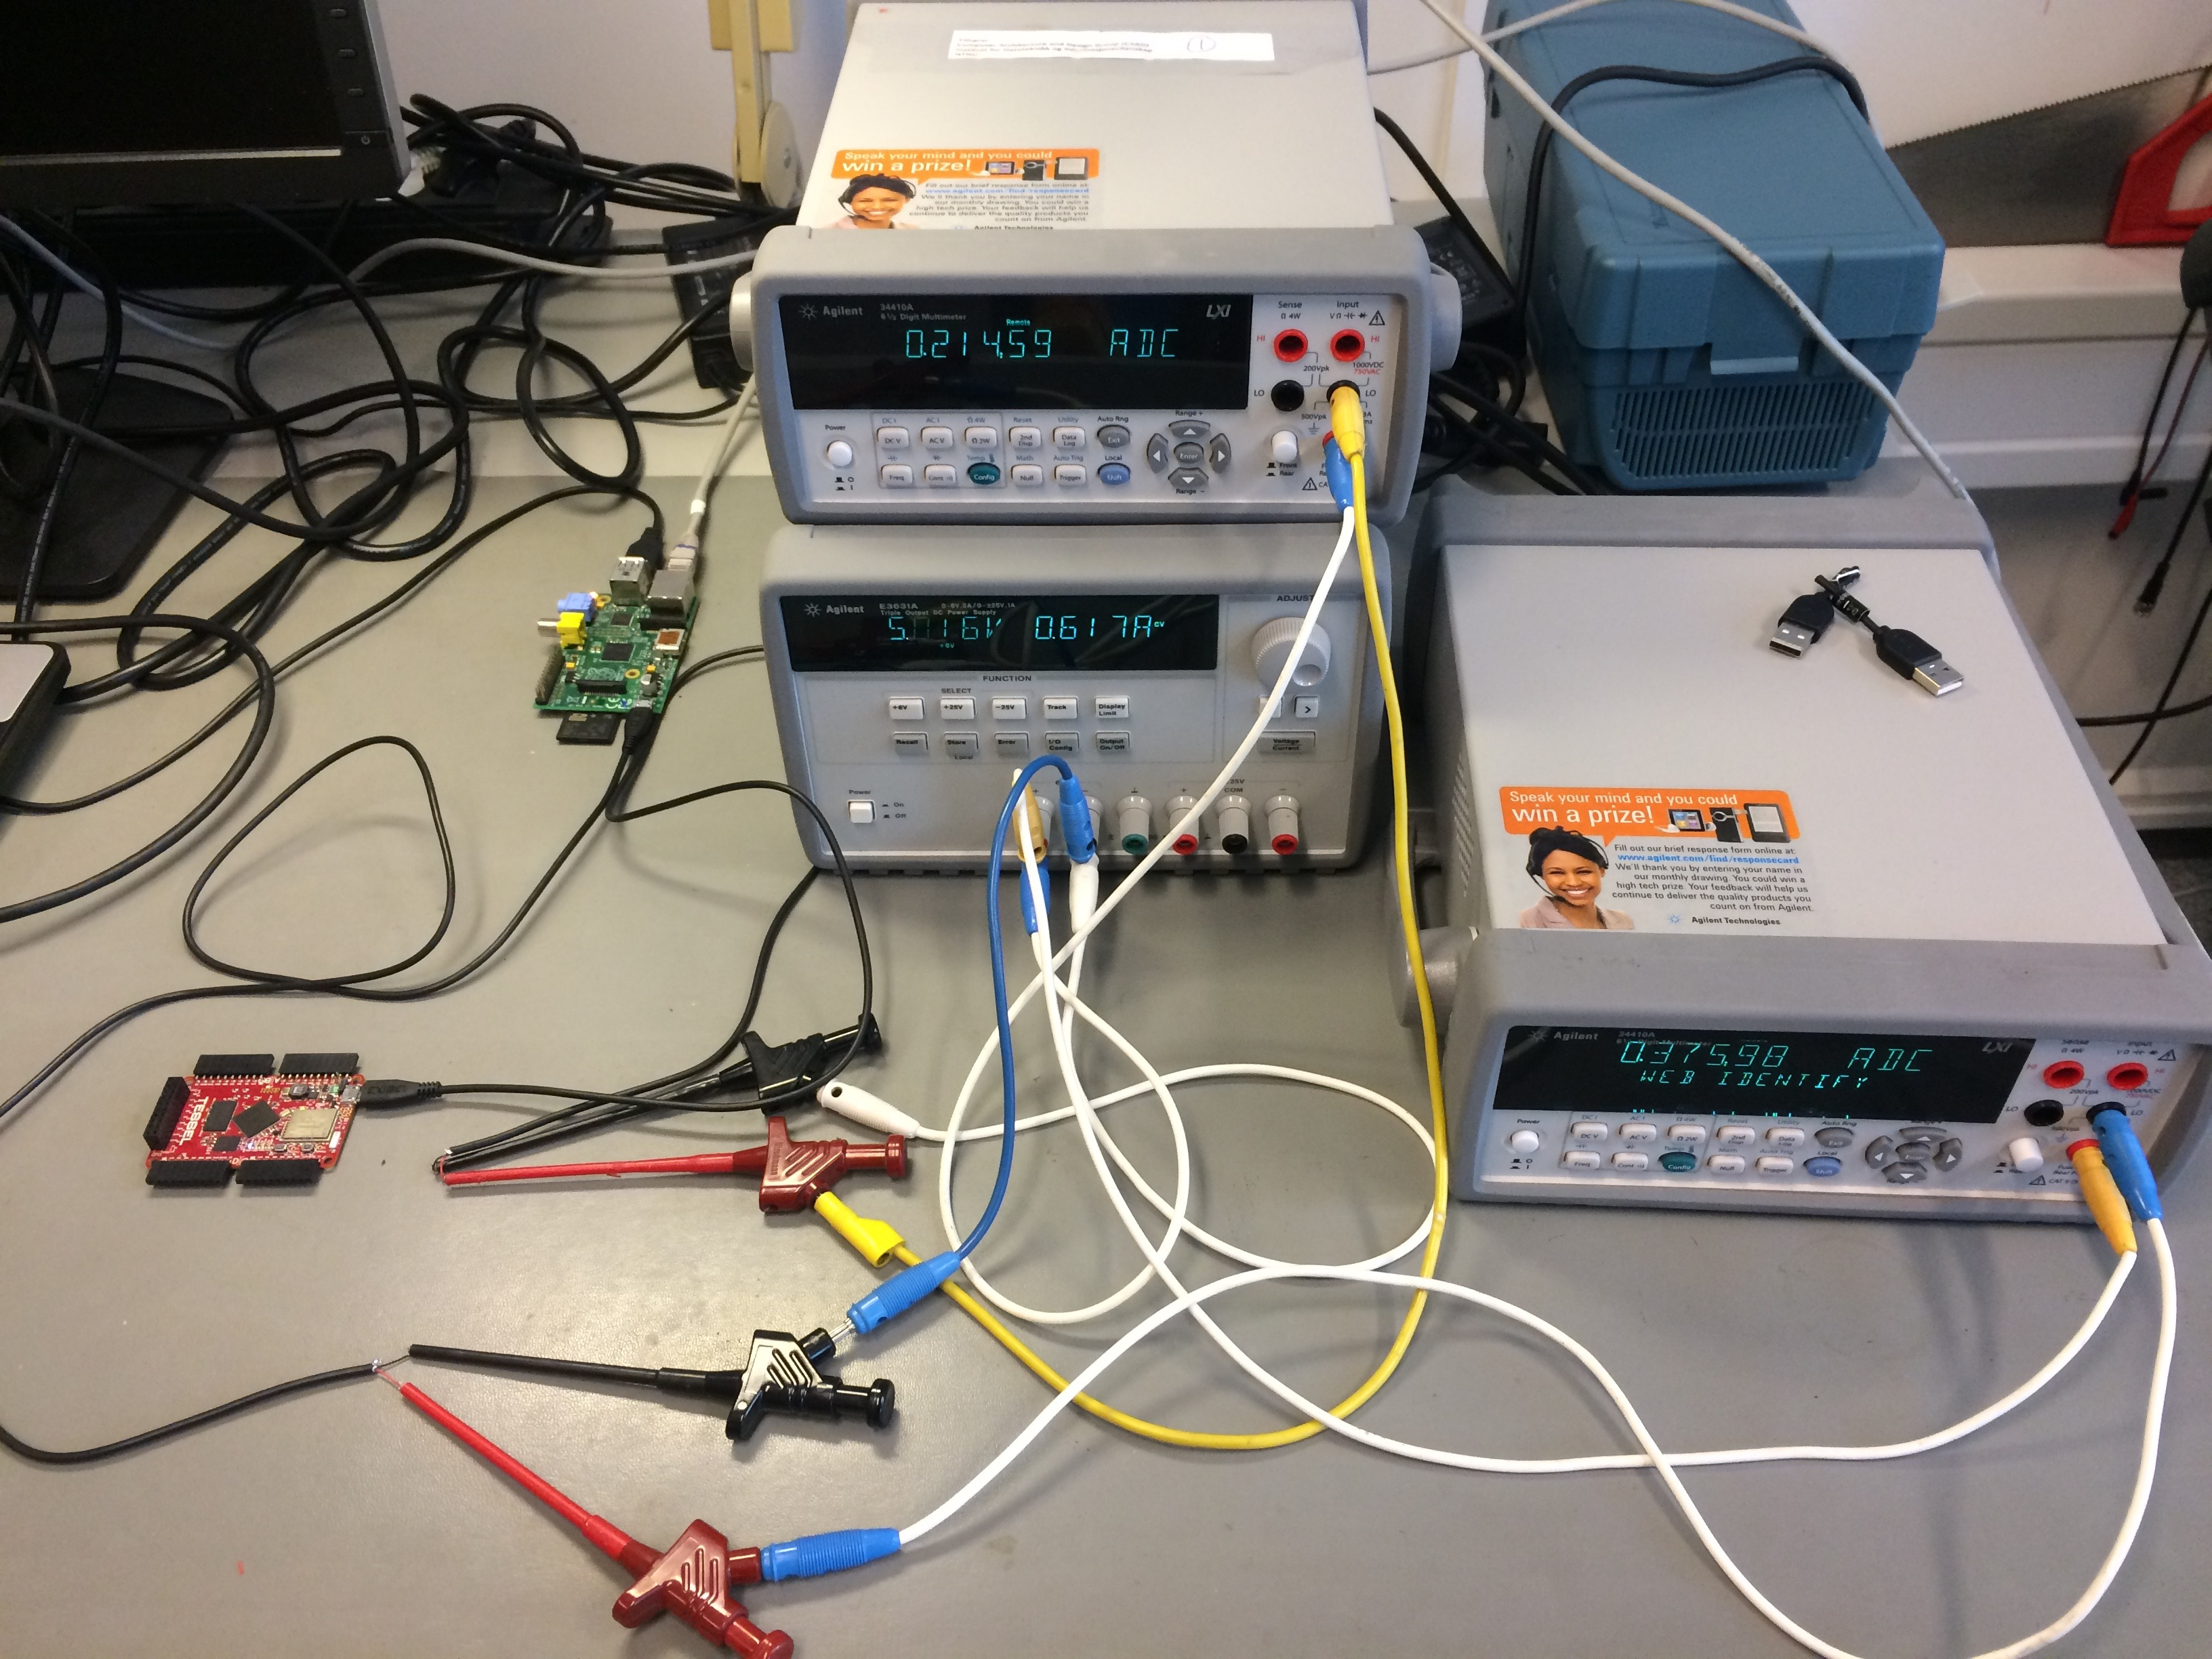
\includegraphics[width=\textwidth]{fig/pics/setup.jpg}
\caption{The hardware setup of the experiment}
\label{fig:setup}
\end{figure}
\defcitealias{usbmicro}{Universal Serial Bus Micro-USB Cables and Connectors Specification, 2007}
To power the experiment, the Keysight E3631A was used. 
As both the hardware platforms were running experiments at the same time, they were both connected to the power supply, with a common ground.
The voltage was set to 5.015\si{\volt}, as it is the recommended operating voltage for the Raspberry Pi, and it is within the supported for the Tessel. 
The multimeter, Keysight 34410A, was connected in series between the power supply and the device, set to ADC measurement. 
%http://www.keysight.com/en/pd-692834-pn-34410A/digital-multimeter-6-digit-high-performance?cc=NO&lc=eng
There was one multimeter for each device while running in parallel.
Both devices receive power through a Micro USB cable.
A cable was cut, and with clamps, the power and ground wires were connected to the power supply.\citepalias{usbmicro}

The multimeter supports logging over LAN, allowing to remotely monitor the experiment.
Using the Keysight Benchvue Software, all measurements can be exported in CSV format.
Together with the Raspberry Pi's remote SSH-access, the experiments on the Pi could be remotely started and controlled.
To fully automate the experiment on the Raspberry Pi, a shell script was written to restart the program as many times as was required in the experiment.
After each run, the device would sleep for 0.5 seconds before the reset, to differ between each run.

Unlike the Raspberry Pi, the Tessel hardware does not allow for remote access while it is running on external power, because the USB port is the only communication port able to flash the Tessel.
To work around this problem, the program was written to the internal flash, which will start to run whenever the Tessel boots.
Then the hardware was reset from software after each program run.
This feature did not exist in the platform, but was written for this experiment, and has since been accepted into the project.\footnote{\url{https://github.com/tessel/t1-firmware/pull/140}}
After the approximate wanted number of runs were done, the logging was stopped.

\subsection{Data manipulation}
The Benchvue Software can export the measurement data in CSV format, in two columns with time stamp and the sampled data at that time.
These files were read in a Python program, which did the manipulations needed on the data.

When the Raspberry Pi was sleeping, the current was always under 0.39 \si{\micro\ampere}, and at all other times it was above.
This was exploited to create a stream with only the samples taken while a program was running.
The stream was the split up into blocks of as many samples as the average program contains.
And adding this blocks up, the energy consumed of one program run was found.
The average of these sums was then the average power usage of one experiment.

To get similar data from the Tessel, the current readings through the reset procedure needed to be stripped away.
As these were not as clear to where started and ended as the dips in the Raspberry Pi, as seen in \cref{fig:multtes}, this was not as easy.
Instead of filtering the data below a threshold, the time data is used to remove the samples after each program has been run, using the approximate running times in \cref{tab:timedruns}, and the timed reset at 12.8 \si{\second}.
Then the samples kept were used in the same manner as for the Raspberry Pi programs.

To show current data for a single iteration in the loop, this sum was divided by 1,000,000, giving the current drawn per iteration.
And the power was calculated using the formula:
\[P = IV\]
Which shows the electric power used by each iteration.